% !TEX root = ../entropy.tex

\section{Methods}%
\label{sec:methods}


\paragraph{Dataset description}
\label{par:dataset_description}

We use data from Money Dashboard (MDB), a financial management app that allows
its users to link accounts from different banks to obtain an integrated view of
their
finances.\footnote{\href{https://www.moneydashboard.com}{https://www.moneydashboard.com}.}
The dataset contains more than 500 million transactions made between 2012 and
June 2020 by about 250,000 users, and provides information such as date,
amount, and description about the transaction as well as account and user-level
information.

The main advantages of the data for the study of consumer financial behaviour
are its high frequency, that it is automatically collected and updated and thus
less prone to errors and unaffected by biases that bedevil survey measures, and
that it offers a view of consumers' entire financial life across all their
accounts, rather than just a view of their accounts held at a single bank,
provided they added all their accounts to MDB. The main limitation is the
non-representativeness of the sample relative to the population as a whole.
Financial management apps are known to be used disproportionally by men,
younger people, and people of higher socioeconomic status
\citep{carlin2019generational}. Also, as pointed out in
\citet{gelman2014harnessing}, a willingness to share financial information with
a third party might not only select on demographic characteristics, but also
for an increased need for financial management or a higher degree of financial
sophistication. Because our analysis does not rely on representativeness, we do
not address this.\footnote{For an example of how re-weighing can be used to
mitigate the non-representative issue, see \citet{bourquin2020effects}.}


\paragraph{Preprocessing and sample selection}%
\label{par:preprocessing_and_sample_selection}

We restrict our sample to users for whom we can observe a regular income, can
be reasonably sure that they have added all their bank account to MDB, and for
whom we observe at least six months of data. Table~\ref{tab:selection}
summarises the sample selection steps we applied to a 1 percent sample of the
raw data, associated data losses, and the size of our final sample. A detailed
description of the entire data cleaning and selection process is provided in
Appendix~\ref{sec:data}.

\begin{table}[H]
\caption{Sample selection}\label{tab:selection}
\begin{tabular}{lrrrr}
\toprule
                                                 &  Users & Accounts & Transactions & Value (\pounds M) \\
\midrule
                                      Raw sample & 24,163 &  123,625 &   59,647,019 &          11,209.7 \\
                       At least 6 months of data & 21,508 &  117,000 &   59,088,076 &          11,116.8 \\
                               No missing months & 18,550 &   98,513 &   51,252,412 &           9,606.4 \\
                      Account balances available & 14,714 &   85,590 &   44,163,629 &           8,618.7 \\
At least 5 debits totalling \pounds200 per month & 12,296 &   70,981 &   38,618,825 &           7,469.7 \\
                    At least one current account & 12,148 &   70,366 &   38,280,116 &           7,421.9 \\
            Income in 2/3 of all observed months &  9,963 &   60,151 &   33,270,455 &           6,490.2 \\
 Yearly income between \pounds5k and \pounds200k &  6,716 &   36,829 &   21,460,727 &           3,677.9 \\
            No more than 10 accounts in any year &  6,169 &   26,999 &   18,241,355 &           2,855.1 \\
      Debits of less than \pounds100k each month &  5,760 &   24,486 &   16,409,561 &           1,998.7 \\
                                    Final sample &  5,760 &   24,486 &   16,409,561 &           1,998.7 \\
\bottomrule
\end{tabular}

\end{table}

\paragraph{Variable description}%
\label{par:dependent_variable}

\paragraph{Outcome variable:}%
\label{par:outcome_variable_}
Our outcome variable is a binary indicator for whether or not a user has made
any payments into their savings accounts in a given month. We classify as
payments into savings accounts all savings account credits of \pounds5 or more
that are not identified as interest payments or automated "save the change"
transfers. While standing order transactions are unlikely to be related to
entropy in the short-run, we do not exclude such transactions since, best we
can tell, the only account for a small fraction of total transactions.


\citet{mps2018building} finds that saving habit is often more important than
amount saved. On individual level, has saving habit dummy as outcome. Could
also use 12-month rolling window.





\paragraph{Variable of interest:}%
\label{par:variable_of_interest_}
Our variable of interest is spending entropy, a measure of how predictable an
individual's spending pattern is at a given point in time, which we interpret
more broadly as a measure of the degree to which an individual's life is
chaotic. Entropy is a cornerstone of information theory, where it measures the
amount of information contained in an event. In the behavioural sciences,
behavioural entropy has recently been shown to predict the frequency of grocery
visits and the per-capita spend per visit \citep{guidotti2015behavioral}, the
amount of calories consumed \citep{skatova2019those}, and the propensity for
financial distress \citep{muggleton2020evidence}.

We calculate spending entropy using the formula proposed by
\citet{shannon1948mathematical}, which defines entropy as:\footnote{Shannon
    entropy is customarily denoted as $H$ following Shannon's own naming after
    Ludwig Boltzman's 1872 H-theorem in statistical mechanics, to which it is
analagous.}

\begin{equation}
\label{equ:entropy}
    H = -\sum{p_i}log(p_i),
\end{equation}

where $p_i$ is the probability that an individual makes a purchase in spending
category $i$, and $log$ is the base 2 logarithm.

\edit{We normalise $H$ by $log(N_{SC})$, the entropy of completely random shopping
    behaviour, so that it takes value between 0 and 1.\footnote{$log(N_{SC})$ is
    the probability of a completely random shopping pattern because for in this
case, for $N_{SC}$ different spending categories, we would have $p_i = 1 /
N_{SC}$ for each category $i$ so that $H = -N_{SC}p_ilog(p_i) = -log(p_i) =
log(N_{SC})$.}}

The higher the value of
entropy, the less predictable an individuals spending pattern.

To calculate entropy scores, we group spending into 9 spending categories (SC)
based on the classification used by Lloyds Banking Group as discussed in
\citet{muggleton2020evidence}. Also following that paper, we use additive
smoothing to calcualte probabilities to avoid taking logs of zeroes in cases
where an individual makes no purchases in a given spending category. We thus calculate $p_i$ as: 

\begin{equation}
    p_i = \frac{\text{Count of purchases in $SC_i$} + 1}{\text{Count of
    all purchases} + N_{SC}},
\end{equation}

where $N_{SC}$ is the total number of categories.

Figure~\ref{fig:entropy} shows the distribution of spending entropy as well as
the distributions of the number of spend transactions, the number of distinct
categories within which these transactions fall, and the proportion of
transactions in each category.

\begin{figure}[H]
    \center \newcommand\width{\textwidth} \caption{Transactions distributions}
    \label{fig:entropy}
    % 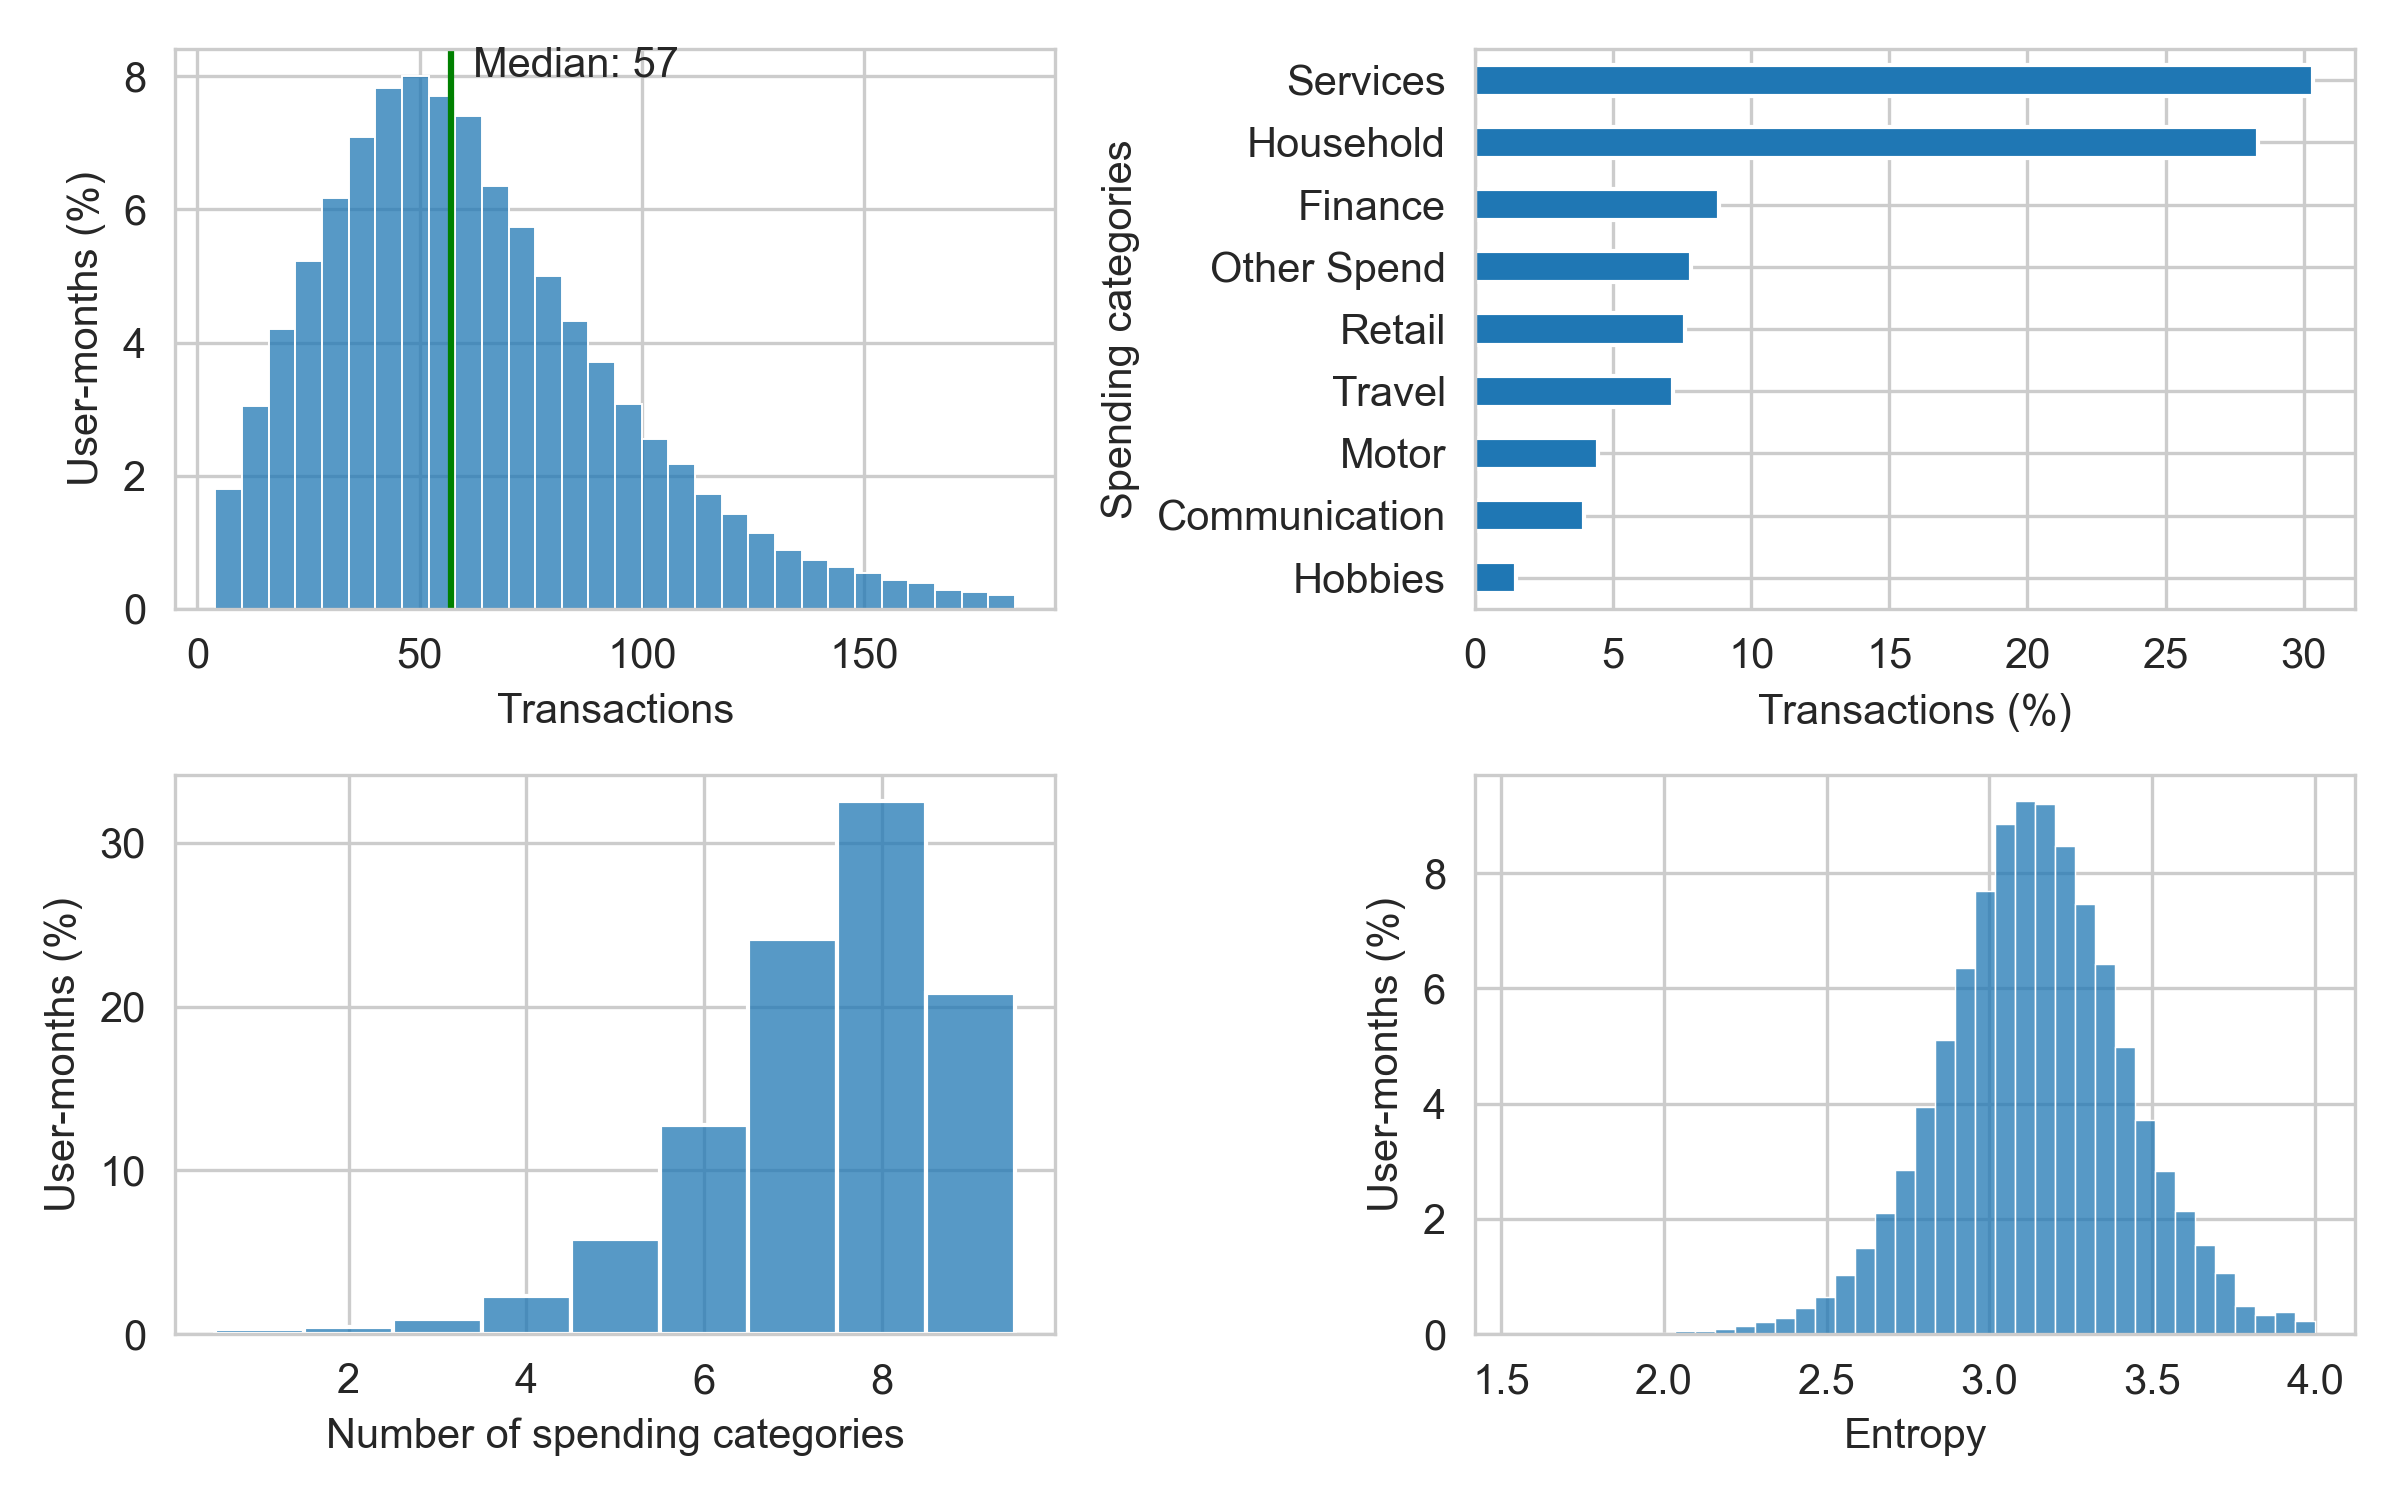
\includegraphics[width=\width]{\figdir/txns_breakdowns_and_entropy.png}
    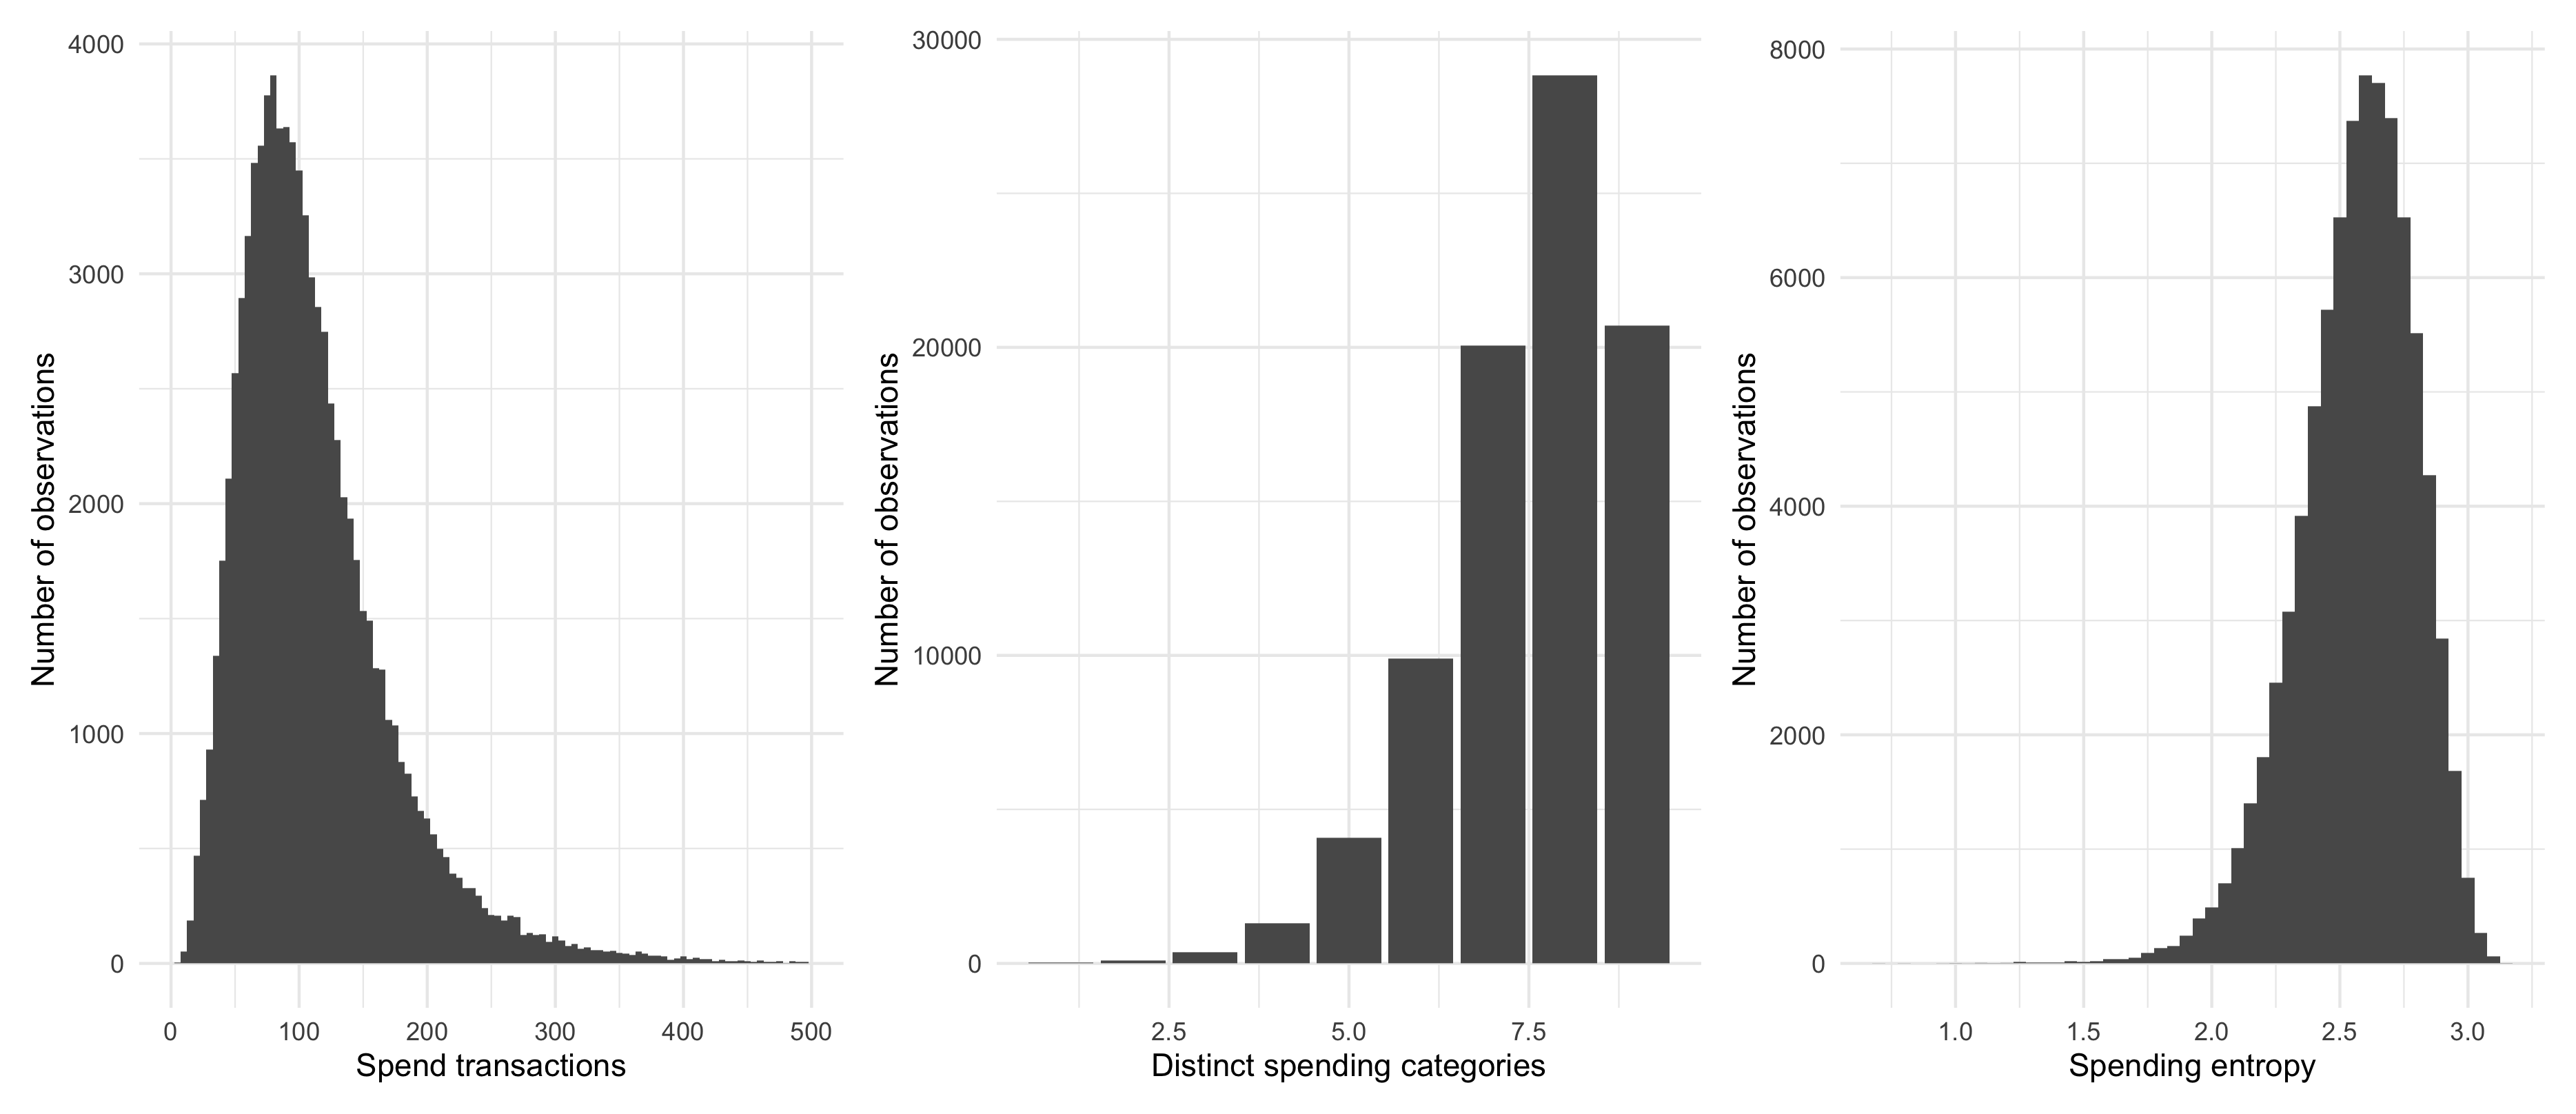
\includegraphics[width=\width]{\figdir/entropy_hists.png}
    \fignote{\width}{From top-left to bottom-right: distribution of spending
    transactions per user-month, breakdown of spending transactions into
spending categories; breakdown of number of spending categories spent on in
user-month; distribution of user-month entropy scores.}
\end{figure}

\paragraph{Auto tag entropy}%
\label{par:auto_tag_entropy}

\begin{itemize}
    \item Use apriori algorithm

    \item minsup: minimum number of baskets a pattern is required to appear
        (else it's dropped)

    \item In our context: baseket is collection of auto tags with positive txsn
        counts in a user month, while pattern is pattern of such auto tags.

    \item Patterns also called 'representative baskets'.

    \item Algorithm steps (adapted from guidotti2015behavioural)

        \begin{itemize}
            \item Identify all patterns (representative baskets)

            \item Discard representative baskets that appear in fewer than
                minsup months we observe for a user. 

            \item Assign representative basked to each of the user's months.

            \item Calculate probabilities of observing a representative basked
                based on occurrences across all of a user's month. E.g. user
                with 5 months of data with representative baskets [1, 1, 2, 3,
                4] has representative basket probabilitis 2/5 for repr basket
                1, and 1/5 for repr baskets 2-4.

            \item Calculate user-leven entropy based on probabilities.
        \end{itemize}
\end{itemize}





\paragraph{Shopping-time based entropy}%
\label{par:shopping_time_based_entropy}

We calculate entropy based on the probability of $(day of week, merchant)$
tuples, where we follow \citet{guidotti2015behavioral} and bin \textit{day of
week} into \textit{weekends} and \textit{weekday}, to reduce excessive
fluctuations. Because banks tend to process weekend transactions on Monday, as shows in
Figure~\ref{fig:dow_txns}, we cannot distinguish transactions made on Saturdays
or Sundays from those made on Mondays, and thus classify all of them as weekend
transactions.

\begin{figure}[H]
    \center \newcommand\width{.7\textwidth} \caption{Transactions by day of week}
    \label{fig:dow_txns}
    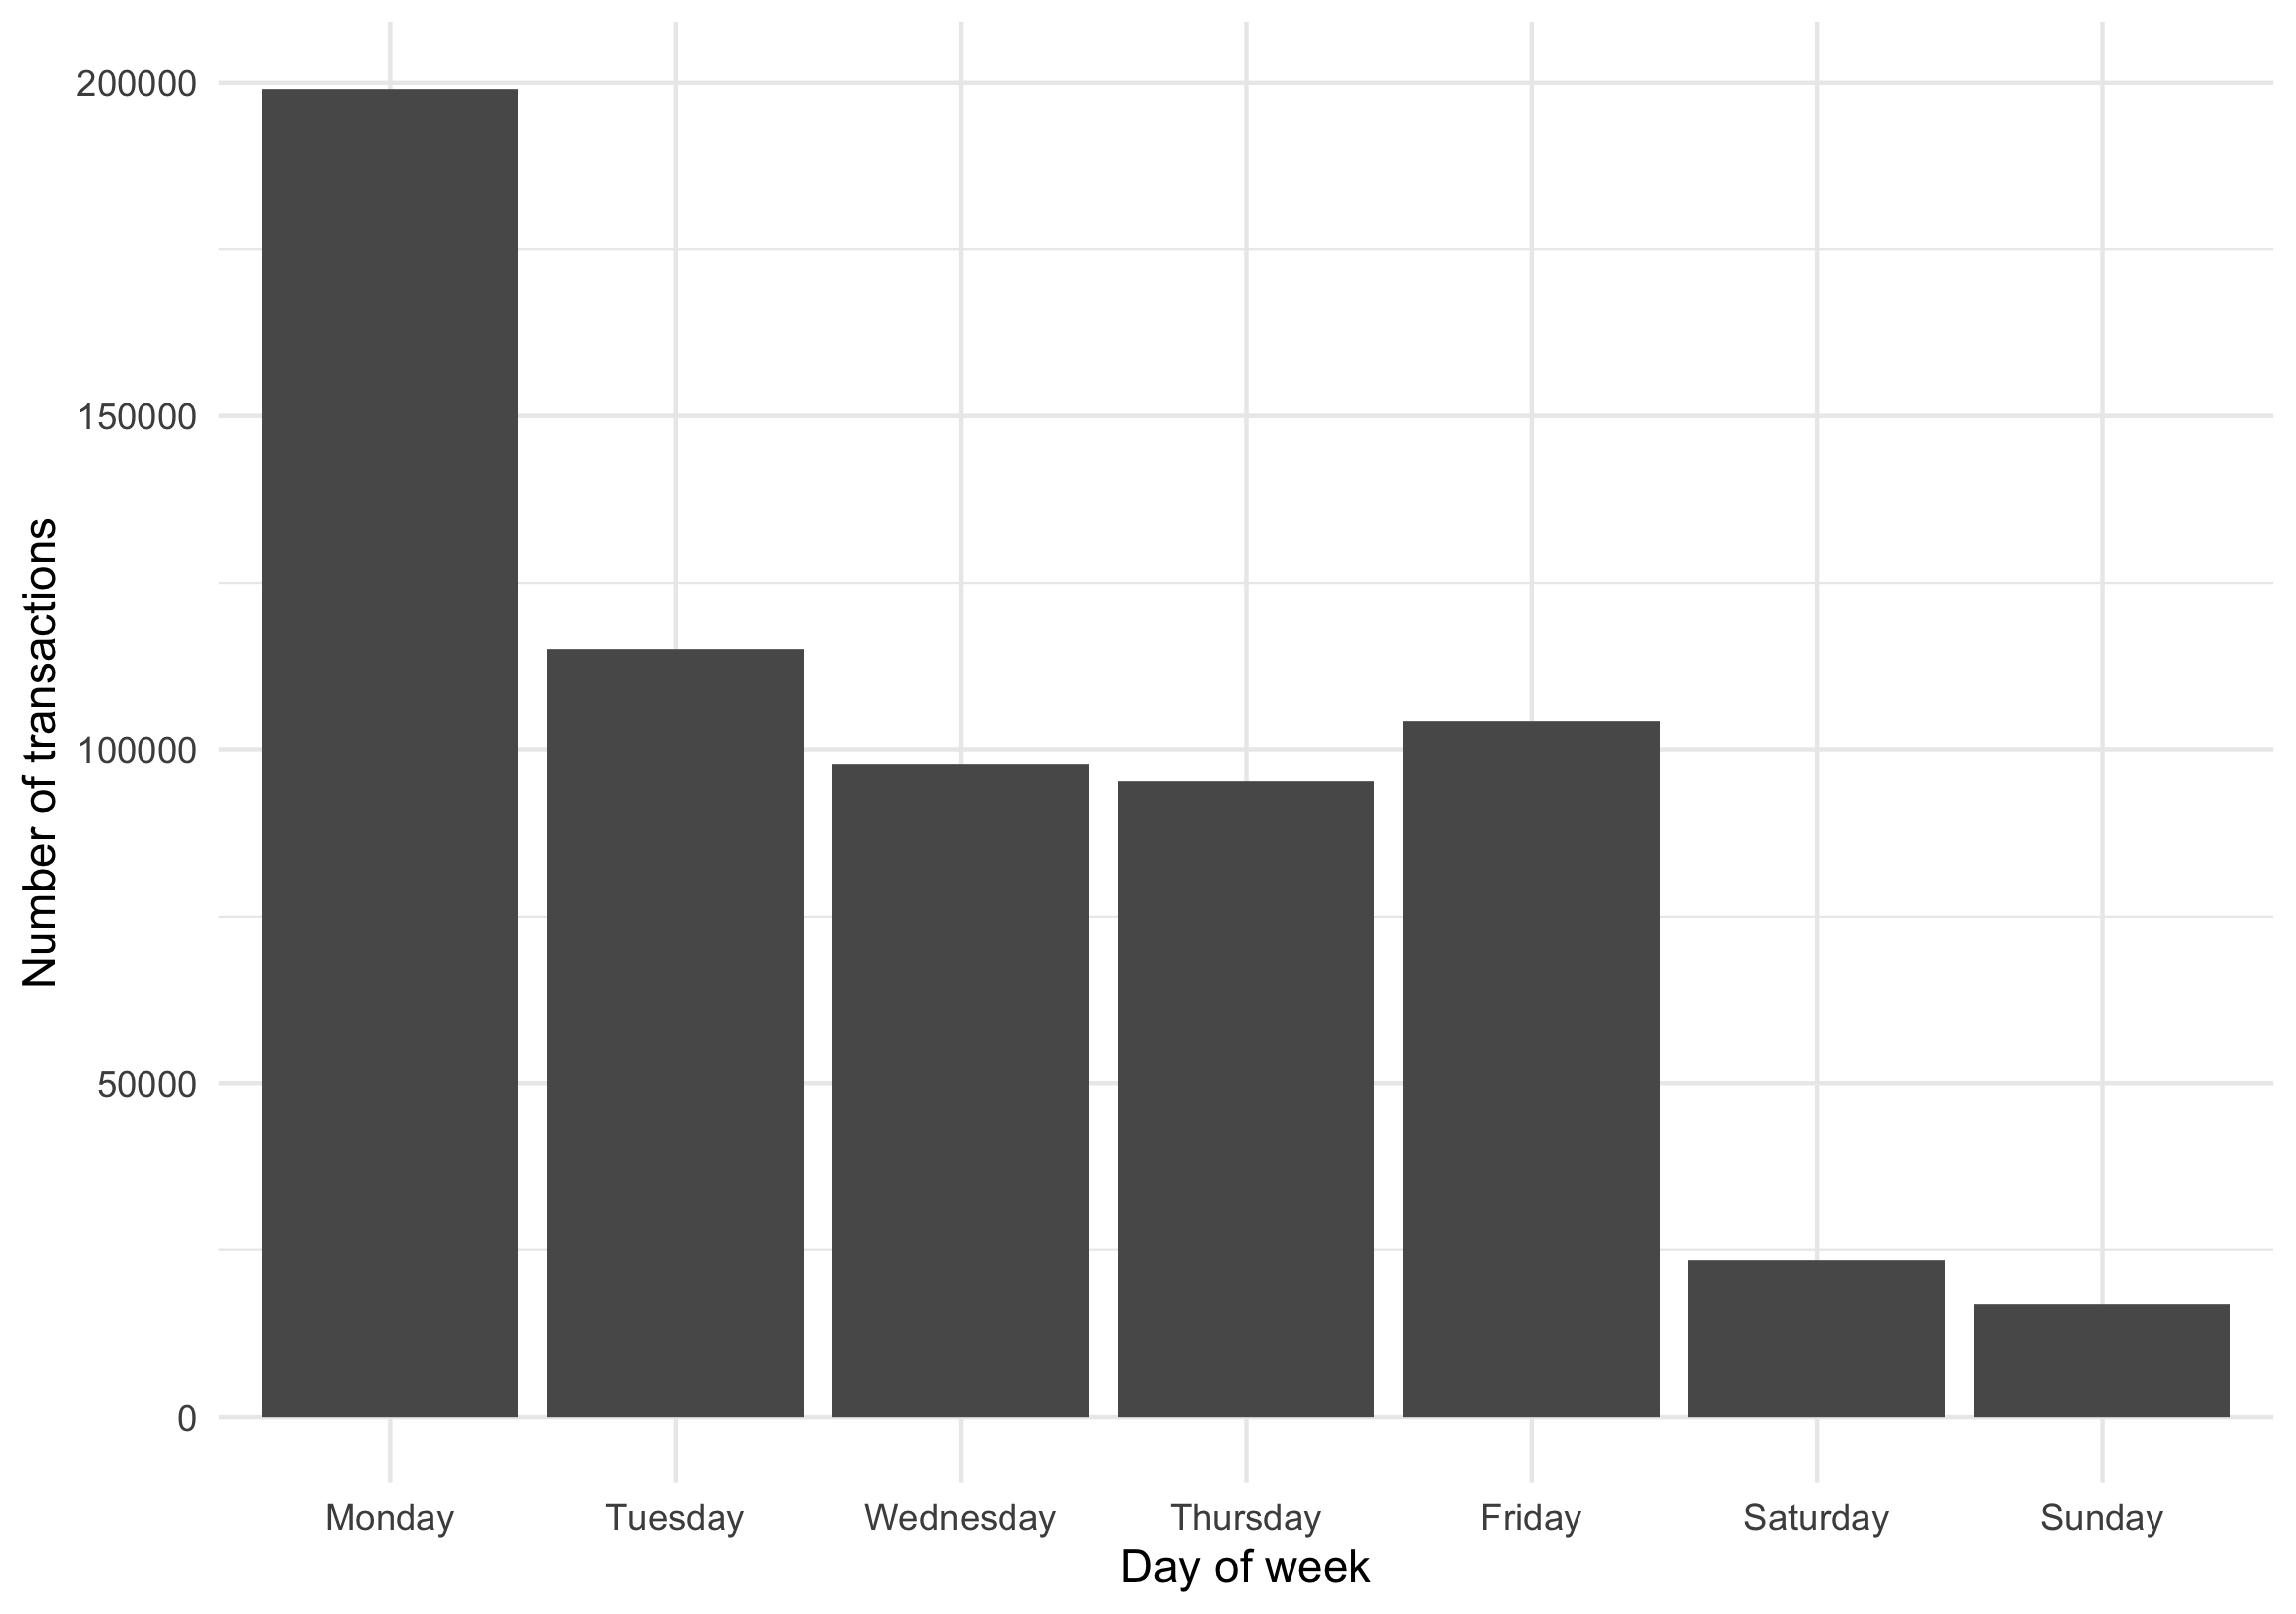
\includegraphics[width=\width]{\figdir/dow_txns.png}
    \fignote{\width}{Number of transactions by day of week, based on a 1/1000
    sample of the full data. Shows that banks process most weekend
transactions on Mondays.}
\end{figure}

We drop the about 25 percent of transactions for which we cannot identify a
merchant. The alternative would be leaving these transactions in the sample and
treating ``unknown merchant'' as a single merchant. But for user-months for
which the merchant is unknown for all transactions, this would lead to an
entropy score of 0, which is undesireable.




% for sequence-dependent entropy, look into krumme2013predictability

\paragraph{Summary statistics}%
\label{par:summary_statistics}
% \begin{table}[H]
% \caption{Summary statistics}\label{tab:sumstats}
% 
% Table created by stargazer v.5.2.3 by Marek Hlavac, Social Policy Institute. E-mail: marek.hlavac at gmail.com
% Date and time: Mon, Sep 26, 2022 - 09:41:15
\begin{tabular}{@{\extracolsep{5pt}}lccccccc} 
\\[-1.8ex]\hline 
\hline \\[-1.8ex] 
Statistic & \multicolumn{1}{c}{Mean} & \multicolumn{1}{c}{St. Dev.} & \multicolumn{1}{c}{Min} & \multicolumn{1}{c}{Pctl(25)} & \multicolumn{1}{c}{Median} & \multicolumn{1}{c}{Pctl(75)} & \multicolumn{1}{c}{Max} \\ 
\hline \\[-1.8ex] 
Month income & 2.77 & 2.23 & 0.00 & 1.45 & 2.18 & 3.43 & 13.69 \\ 
Has income in month & 0.98 & 0.13 & 0 & 1 & 1 & 1 & 1 \\ 
Has savings & 0.50 & 0.50 & 0 & 0 & 1 & 1 & 1 \\ 
Month spend & 2.90 & 2.50 & 0.20 & 1.37 & 2.20 & 3.49 & 16.05 \\ 
Age & 35.72 & 9.74 & 18 & 28 & 34 & 42 & 65 \\ 
Female & 0.43 & 0.49 & 0 & 0 & 0 & 1 & 1 \\ 
Urban & 0.85 & 0.36 & 0 & 1 & 1 & 1 & 1 \\ 
Unique categories (9) & 7.84 & 1.05 & 1 & 7 & 8 & 9 & 9 \\ 
Unique categories (48) & 16.54 & 4.13 & 1 & 14 & 16 & 19 & 35 \\ 
Unique categories (Merchants) & 26.78 & 9.35 & 2 & 20 & 26 & 33 & 85 \\ 
\hline \\[-1.8ex] 
\end{tabular} 

% \end{table}

\paragraph{Model specification}%
\label{par:model_specification}

We estimate models of the form: 

\begin{equation}
    s_{i,t} = \alpha_i + \lambda_t + \beta H_{i,t} + x^\prime_{i,t} \delta +
    \epsilon_{i,t},
\end{equation}

where $s_{i,t}$ is an indicator variable equal to one if individual $i$ made
one or more transfers to any of their savings account in month $t$ and zero
otherwise, $H_{it}$ is $i$'s spending entropy in month $t$,
$x_{i,t}$ a vector of control variables, $\alpha_i$ an individual fixed effect, $\lambda_t$ a calendar
month fixed effect, and $\epsilon_{i, t}$ the error term.
